\documentclass[11pt,compress,t,notes=noshow, xcolor=table]{beamer}


\input{../../style/preamble}
\input{../../latex-math/basic-math}
\input{../../latex-math/basic-ml}

\setbeamersize{text margin left=0.3cm,text margin right=0.3cm}


\title{Applied Machine Learning}
% \author{LMU}
%\institute{\href{https://compstat-lmu.github.io/lecture_iml/}{compstat-lmu.github.io/lecture\_iml}}
\date{}

\begin{document}

\titlemeta{
Time Series:
}{
Introduction and Forecasting Setup
}{
figure/bike_one_week
}{
\item What is a time series?
\item Tree-based models for time series
\item Detrending and multi-step forecasting
}

\begin{vbframe}{Running Example: The Bike Sharing Dataset}
\vfill
Hourly bike rental data from Washington D.C.
\vfill
\scriptsize
\begin{tabular}{lllrrrlr}
\toprule
holiday & workingday & weather & temp & humidity & windspeed & datetime & count \\
\midrule
False & False & clear & 9.84 & 0.81 & 0.00 & 2011-01-01 00:00 & 16 \\
False & False & clear & 9.02 & 0.80 & 0.00 & 2011-01-01 01:00 & 40 \\
False & False & clear & 9.02 & 0.80 & 0.00 & 2011-01-01 02:00 & 32 \\
False & False & clear & 9.84 & 0.75 & 0.00 & 2011-01-01 03:00 & 13 \\
False & False & clear & 9.84 & 0.75 & 0.00 & 2011-01-01 04:00 & 1 \\
\bottomrule
\end{tabular}
\vfill
\pause
Task: Predict hourly rental count
\pause
Question: how to feed this to a standard ML model?
\vfill
\end{vbframe}

\begin{vbframe}{What Does the Data Look Like?}
\vfill
\begin{center}
  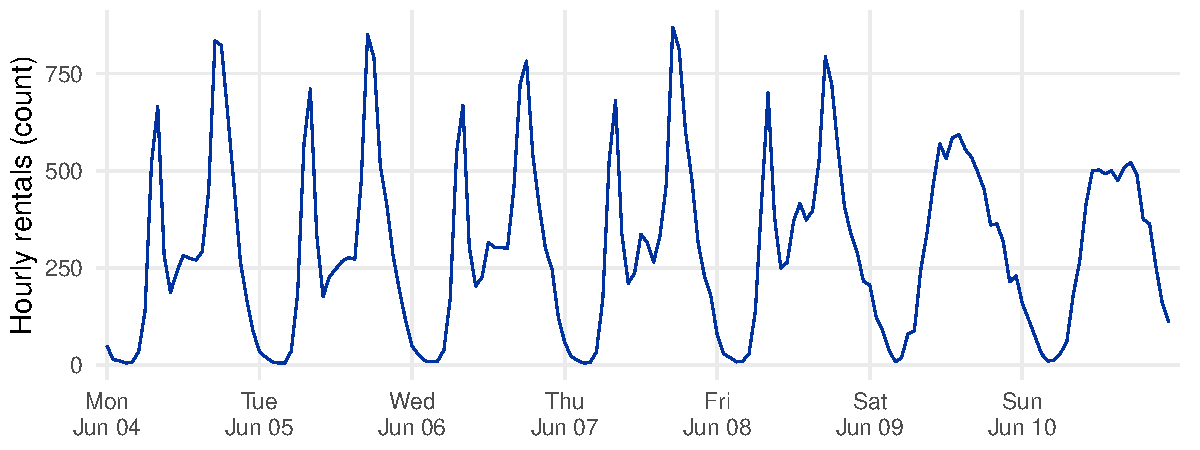
\includegraphics[width=0.95\textwidth]{figure/bike_one_week.pdf}
\end{center}
\vspace{-0.5em}
\footnotesize
Hourly bike rentals -- one week in June 2012. Notice: \textbf{daily seasonality} (commuter peaks at 8am/5pm on weekdays) and \textbf{weekly seasonality} (smooth single-peak pattern on Sat/Sun).
\vfill
\end{vbframe}

\begin{vbframe}{Key Definitions}
  \begin{itemize}
    \item \textbf{Time series} $\{y_t\}_{t=1}^{T}$: ordered observations indexed by time:
    \begin{itemize}
        \item Timestamps - Specific instants in time.
        \item Fixed periods - Such as the whole month of January 2017, or the whole year 2020.
        \item Intervals of time - Indicated by a start and end timestamp. Periods can be thought of as special cases of intervals.
        \item Experiment or elapsed time - Each timestamp is a measure of time relative to a particular start time (e.g., the diameter of a cookie baking each second since being placed in the oven), starting from 0.
    \end{itemize}
    \item \textbf{Exogenous variable / covariate}: external feature $x^{(j)}_t$ influencing $y_t$
    \item \textbf{Trend}: long-term increase or decrease
    \item \textbf{Seasonality}: systematic, calendar-related patterns
    \item \textbf{Stationarity} (briefly): distribution of $y_t$ does not change over time
  \end{itemize}
\end{vbframe}

\begin{vbframe}{Tasks}
\vfill
    \begin{itemize}
        \item \textbf{Time Series Analysis}

        Decompose time series into trend, seasonality, and residuals for understanding $\rightarrow$ time series course

        \item \textbf{Time Series Forecasting}

        Fit a model on historical data and make predictions about the future.

        \item \textbf{Time Series Classification}

        Classify entire time series recordings, e.g., classify sensor signals as normal vs.\ faulty.

        \item \textbf{Anomaly Detection}

        Identify unusual observations or subsequences, e.g., fraud detection, sensor fault monitoring.
    \end{itemize}
\vfill
\end{vbframe}

\begin{vbframe}{How to Tackle Time Series Forecasting?}
\vfill
    \begin{itemize}
        \item \textbf{Statistical Models}

        ARIMA, ETS (Error, Trend, Seasonality) $\rightarrow$ time series course

        \item \textbf{Recurrent Models}

        Deep learning architectures that track the state of data over time $\rightarrow$ deep learning lecture

        \item \textbf{Transformer Models}

        Attention-based architectures for sequential data $\rightarrow$ deep learning lecture

        \item \textbf{Feature Engineering + Standard ML Models}

        Engineer temporal features (lags, rolling stats, calendar) from the time index and feed them to standard ML models (e.g., gradient boosting). $\rightarrow$ \textbf{focus of this lecture}
    \end{itemize}
\vfill
\end{vbframe}

\begin{vbframe}{Why Tree-Based Models for Time Series?}
\vfill
With proper feature engineering, standard tabular ML models work surprisingly well for time series forecasting:
\vfill
\begin{itemize}
    \item Handle mixed feature types naturally (calendar integers + continuous weather data)
    \item No stationarity assumptions required (unlike ARIMA)
    \item Fast to train and easy to tune
    \item Feature engineering makes temporal patterns accessible to non-temporal models
    \item Very competitive in Kaggle competitions and industry (e.g., gradient-boosted trees were widely used in top M5 forecasting competition solutions, often in ensembles\footnote{\tiny\url{https://mofc.unic.ac.cy/m5-competition/}})
\end{itemize}
\vfill
\textbf{Caveat:} Tree-based models cannot extrapolate beyond the training range. If the data has a strong upward trend, predictions will plateau. See the next slide for how to handle this.
\vfill
\end{vbframe}

% See rsrc/detrending_mlr3.R for a full mlr3 implementation of leakage-safe
% detrending via PipeOpTargetTrafo (based on https://chatgpt.com/share/69dc97c5-ea14-838f-9a42-5aa4c7cba008)
\begin{vbframe}{Detrending for Tree-Based Models}
\begin{center}
  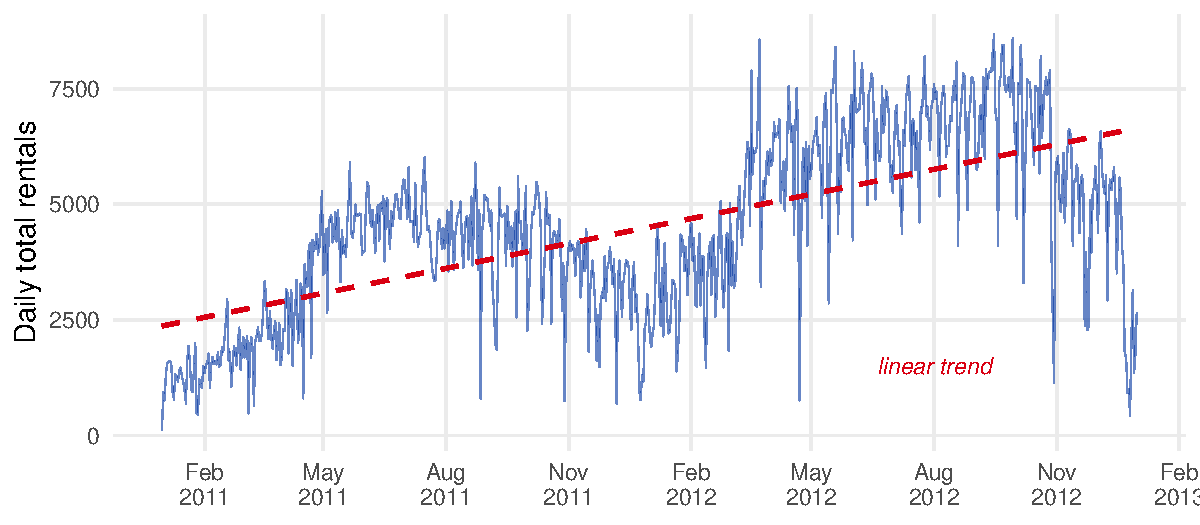
\includegraphics[width=0.65\textwidth]{figure/bike_trend.pdf}
\end{center}
\vspace{-0.8em}
\footnotesize
\begin{enumerate}\setlength{\itemsep}{1pt}
    \item Fit a trend model on the \textbf{training fold only} (e.g., linear regression on the time index)
    \item Subtract the trend from training targets: $r_t = y_t - \hat{\text{trend}}_t$
    \item Train the tree model on the residuals $r_t$
    \item At prediction time: extrapolate the trend, predict residuals, add them: $\hat{y}_t = \hat{r}_t + \hat{\text{trend}}_t$
\end{enumerate}
\vspace{0.3em}
\textbf{Important:} this is a target transformation and must be part of the modelling pipeline. The trend must be re-estimated on each training fold; detrending on the full dataset before splitting leaks future information and makes CV results overly optimistic.\\
Alternative: use differencing ($y_t - y_{t-1}$) as the target, which also removes linear trends.
\vfill
\end{vbframe}

\begin{vbframe}{Multi-Step Forecasting Strategies}
\vfill
How to predict multiple steps ahead (e.g., the next 168 hours)?
\vfill
\begin{itemize}
    \item \textbf{Recursive:} train a 1-step model, feed its prediction as input for the next step, repeat
    \begin{itemize}
        \item Simple, but errors accumulate over the horizon
    \end{itemize}
    \item \textbf{Direct:} train a separate model for each horizon ($h=1, 2, \ldots, H$)
    \begin{itemize}
        \item No error accumulation, but $H$ models to train and no shared learning
    \end{itemize}
    \item \textbf{Multi-output:} single model predicts all $H$ horizons at once
    \begin{itemize}
        \item Efficient, but requires a model that supports vector output
    \end{itemize}
    \item \textbf{DirRec (hybrid):} train a direct model for each horizon, but include recursive predictions from earlier horizons as additional features
\end{itemize}
\vfill
\end{vbframe}


\endlecture
\end{document}
